%% LyX 1.3 created this file.  For more info, see http://www.lyx.org/.
%% Do not edit unless you really know what you are doing.
\documentclass[frenchb,titleabove,10pt,contbibnum]{cv}
%\usepackage[numbers,sort&compress]{natbib}%
%%%%%%%%%%%%%%%%TRUCS FRANCAIS
\clubpenalty=10000
\widowpenalty=10000
\brokenpenalty=10000
  \hyphenpenalty=5000
  \tolerance=1000
\sloppy
\usepackage[cyr]{aeguill}
\setlength{\parindent}{0in}
%\usepackage{enumitem}
%\setlist{nolistsep}
\usepackage{verbatim}
\usepackage{amsmath}
\usepackage{longtable}
\usepackage[english,frenchb]{babel}
%\addto\captionsfrenchb{\renewcommand{\refname}{\vspace{-14pt}}}% can be bibname
%\addto\captionsfrenchb{\renewcommand{\refname}{\vspace{-14pt}}}% can be bibname
%\addto\captionsfrenchb{\renewcommand{\refname}{Bibliographie}}% can be bibname
%\renewcommand{\contentsname}{Sommaire} % si tableofcontents au début
%\newcommand{\Numero}{\No}
%\newcommand{\numero}{\no}
%\newcommand{\fup}[1]{\up{#1}}
%%% N'oubliez pas les espaces devant les doubles ponctuations
\NoAutoSpaceBeforeFDP
%\renewcommand \thesection{\arabic{section}.}
%\renewcommand{\thesubsection}{\arabic{section}.\arabic{subsection}}
%\setcounter{secnumdepth}{2}
%%%%%%%%%%%%%%%%%%FIN TRUCS





\makeatletter

%%%%%%%%%%%%%%%%%%%%%%%%%%%%%% LyX specific LaTeX commands.
%% Because html converters don't know tabularnewline


%%%%%%%%%%%%%%%%%%%%%%%%%%%%%% User specified LaTeX commands.
%% You can modify the fonts used in the document be using the
%% following macros. They take one parameter which is the font
%% changing command.
%% \headerfont: the font used in both headers.
%%              Defaults to sans serif.
%% \titlefont:  the font used for the title.
%%              Defaults to \LARGE sans-serif semi bold condensed.
%% \sectionfont: the font used by \section when beginning a new topic.
%%              Defaults to sans-serif semi bold condensed.
%% \itemfont:   the font used in descriptions of items.
%%              Defaults to sans-serif slanted.
% to make your name even bigger, uncomment the following line:
% \titlefont{\Huge}
%%
%% You can modify the following parameters using \renewcommand:
%% \topicmargin: the left margin inside topics.
%%               Defaults to 20% of the text width (0.20\textwidth).
% To get more room for left column of Topic layouts, uncomment following line:
% \setlength{\topicmargin}{0.3\textwidth}
%\usepackage{epsfig}
%\usepackage{amsmath,amssymb}
%\usepackage{pslatex}
\usepackage{color}

\usepackage{thumbpdf}
 \usepackage[pdftex,urlcolor=black,colorlinks=false]{hyperref}
 \pdfinfo{
            /Title      (C.v. de  Daniel Lemire)
            /Author     (Daniel Lemire, Ph.D.)
            /Subject  (Publications et expériences de Daniel Lemire.)
            /Keywords   ()
          }





%\usepackage{babel}
\makeatother
\begin{document}

\title{Daniel Lemire}
%\rightheader{
%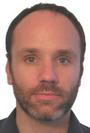
\includegraphics[scale=0.3]{../../images/JPG/profile2004.jpg}%zel4.jpg}
%}
\leftheader{
Centre de recherche LICEF\\
TÉLUQ, Université du Québec\\
%UER Sciences et Technologies, TÉLUQ\\
Pavillon  Saint-Urbain\\
%Université du Québec à Montréal (UQAM)\\
5800, rue Saint-Denis\\
Bureau 1105\\
Montréal (Québec)\\
H2S 3L5 Canada}
\rightheader{
lemire@gmail.com\\
\url{http://lemire.me/fr/}\\
~\\
Citoyen canadien
}

\maketitle

%\textbf{Mots-clefs}~: gestion collaborative des données, theorie des bases de données, entrepôts de données et OLAP, exploration des données (data mining), séries temporelles et chronologiques, filtrage collaboratif, recherche d'informations.

\section{Expérience }

\begin{topic}

\item [2004--\ldots] Professeur d'informatique\\
Centre de recherche LICEF, TÉLUQ, Université du Québec\\
Titularisé en 2009%\\
%TÉLUQ, \textbf{Université du Québec à Montréal (UQAM)}
%\url{http://www.professeurs.uqam.ca/pages/lemire.daniel.htm}





\item [2002--2004] Chercheur régulier en affaires électroniques\\
%Institut de technologie de l'information\\
Conseil national de recherches du Canada (CNRC)%~\footnote{Le CNRC est la plus grande institution de recherche au Canada.}
\\
Chef de l'équipe de recherches en santé électronique (2002--2003)

\item [2001--2002] Professeur adjoint\\
%Département de mathématiques et de statistiques\\
Acadia University


\item [1999--2001] Entrepreneur \\
%Traitement du signal numérique (imagerie médicale et géophysique)\\
TechElements Inc. et Ondelette.com

\item [1998--1999] Stagiaire postdoctoral\\
%Traitement du signal  (ECG, EEG) \\
Institut de génie biomédical
\end{topic}

\section{Formation}

\begin{topic}
\item [1995--1998] Doctorat (Ph.D.) --
\emph{Schémas itératifs}\\ %  en mathématiques de l'ingénieur\\
%Département de mathématiques et génie industriel \\
%<<~Schémas itératifs et ondelettes~>> \\
\textbf{École Polytechnique de Montréal} et \textbf{Université de Montréal}\\
Directeurs~: Prof. Gilles Deslauriers et Serge Dubuc

\item [1994--1995] Maîtrise --
\emph{Approximation dans les systèmes non linéaires}\\
\textbf{University of Toronto}\\
Directrice~: Catherine Sulem

\item [1990--1994]Baccalauréat avec mention \emph{High Distinction}\\
\textbf{University of Toronto}
\end{topic}

\section{Bourses et prix d'excellence à titre d'étudiant}
\begin{itemize}
\item Bourse d'étude du FCAR (doctorat) et CRSNG  (maîtrise et doctorat);
\item Bourse \emph{C. D. Howe Memorial} ($\approx$50~000~\$);
\item Bourse Canada du CRSNG (4~000~\$);
\item Médaille du doyen de St.Michael's (1994);
\item Bourse 3T0 (Université de Toronto). % (1~000~\$).
\end{itemize}

\section{Autres affiliations}
\begin{itemize}
\item Je suis professeur associé à l'Université du Nouveau-Brunswick % au département d'informatique et de statistiques appliquées
et à l'Université du Québec à Montréal où je dirige des étudiants aux cycles supérieurs.
\end{itemize}

\section{Activités d'enseignement récentes}

Premier cycle:
\begin{itemize}
\item INF 1250 - Introduction aux bases de données;
\item INF 6460 - Recherche et filtrage d'informations;
\item INF 6450 - Gestion de l'information avec XML;
\item INF 9002 - Évaluation et analyse des systèmes d'information;
\item INF 9004 - Informatique des entrepôts de données.
\end{itemize}

Cycles supérieurs:
\begin{itemize}
\item INF 6104 - Recherche d'informations et web;
\item INF 6107 - Le Web social;
\item INF 6408 - Informatique de l'analyse multidimensionnelle.
\end{itemize}

De plus, j'ai dirigé et codirigé plusieurs programmes incluant deux certificats,
un baccalauréat, et quatre programmes aux cycles supérieurs
dont la maîtrise en technologie de l'information.

\section{Participation au sein d'associations professionnelles}
\begin{itemize}
\item Association for Computing Machinery (ACM).
%\item ACM Special Interest Group on Electronic Commerce.
%\item ACM Special Interest Group on Information Technology Education.
%\item Institute of Electrical and Electronics Engineers, Inc. (IEEE).
%\item Society for Industrial and Applied Mathematics (SIAM).
%\item W3Québec
%\item Canadian Semantic Web Interest Group (SWIG), premier membre fondateur.
%\item Canadian Society for the Computational Studies of Intelligence (CSCSI)
%\item La Société Québécoise d'Informatique Biomédicale et de la Santé (SoQibs).
\end{itemize}


\begin{comment}
\section{Supervision d'étudiants et de stagiaires}

%En cours~:
\begin{itemize}
\item Ali Assi (Ph.D., 2012--\ldots);
\item Ferenc Molnar (M.Sc., 2012--\ldots)
\item Samy Chambi (Ph.D., 2012--\ldots);
\item Kenza Sakout Andaloussi (Ph.D., 2012--\ldots);
\item Tarek Khei (Ph.D., 2012-\ldots);
\item Ludovic Bocken (Ph.D., 2011--\ldots);
\item Badis Merdaoui (Ph.D., 2008--\ldots).
\item Rohit Patidar (M.Sc., 2012--\ldots);
\item Kushal Mehra (M.Sc., 2012--\ldots);
\item Danièle Massicotte (M.Sc., 2012--\ldots);
\item Charbel Matni (M.Sc., 2011--\ldots);
\item Djamel Garar (M.Sc., 2011--\ldots);
\item Sahbi Khtatfa (M.Sc., 2011--\ldots);
\item Toufik Lazri (M.Sc., 2010--\ldots);
\item Julien Marais (M.Sc., 2011--\ldots);
\item Ikhtear Sharif (M.Sc., 2011--\ldots).
\end{itemize}

Diplômés récents~:
\begin{itemize}
\item
\item Hamid Douzi (D.E.S.S., 2010--2011) est dévelopeur en intelligence d'affaire chez  IMBD (Montréal, Canada);
\item Hazel Webb (Ph.D., 2005--2010) est professeure adjointe  à l'Université du Nouveau-Brunswick (Saint-Jean, Canada);
\item Idris Laabassi (Master, 2010) est gestionnaire des ventes et des technologies de l'information chez OTIS (Libye);
\item Minfang Tao (Stagiaire master, 2011) est analyste d'affaire chez BundleRank.
\item Kamel Aouiche (Postdoct., 2006--2008) est consultant chez Objet direct (Lyon, France);
\item Steve Keith (M.Sc., 2004--2006) est architecte de base de données chez Innovatia (Saint-Jean, Canada).
\end{itemize}

\end{comment}

% Durant le trimestre d'été 2003, Sean McGrath, un étudiant de l'Université
% du Nouveau-Brunswick s'est joint à nous pour travailler sur le projet
% Lemur. Le projet Lemur est un logiciel écrit en C++ et Python pour
% les calculs rapides sur les cubes de données. J'ai ensuite cosupervisé Sean
% avec Harold Boley sur le projet \textit{RACOFI Composer}, et finalement, j'ai
% payé Sean à même ma subvention du CRSNG pour qu'il revienne avec nous
% pour un troisième trimestre. Un des résultats de ces
% travaux fut le site web inDiscover (http://www.indiscover.net).
%
% Durant le trimestre d'hiver 2003, j'ai supervisé Nancy Howse de l'Université
% Acadia dans le cadre de son programme d'étude COOP. Le projet avait
% comme titre: Scale and Translation Invariant Collaborative Filtering
% Systems. Le projet se nommait \textit{COFI Music} et était un sous-projet
% du projet \textit{Sifter} avec Mosaic Corporation. Suite au succès de ce premier
% stage, Nancy est revenue pour un second stage durant l'été 2003. Le
% résultat de son stage est un site web avec servlet (racofi.elg.ca) illustrant
% une application de la théorie. Depuis février 2005, Nancy Howse travaille
% pour Blue Cross à Halifax.
%
%
%%J'ai l'habilitation à la direction d'étudiants au doctorat en informatique et au
%%doctorat en informatique cognitive à l'UQAM. %J'ai l'habilitation à la codirection d'étudiants
%à l'Université du Nouveau-Brunswick.
%Plusieurs de mes communications, articles et rapports furent écrits avec mes étudiants et stagiaires~\cite{elearningsummit, COLA2003, elearningsummitpaper, TRD01, BELL2004-TR,TRD05001,apics2005,kamel1,dolap2007}.
% \begin{small}\begin{center}\begin{longtable}{|p{0.2\columnwidth}|c|c|}
% \hline
% Nom&
% Période&
% Programme\tabularnewline
% \hline
% Nacima Hassaine &
% 2010--\ldots &
% M.Sc.  \tabularnewline
%  Idris Laabassi
% &
% 2010 &
% Stagiaire master (Lyon 2)   \tabularnewline
% Loukmane Arzim &
% 2010--\ldots &
% Ph.D.   \tabularnewline
% Eduardo Gutarra &
% 2010--\ldots &
% M.Sc.   \tabularnewline
% %Wilfrid Blais &
% %2009--\ldots &
% %Ph.D. \tabularnewline
% %Komi Sodoké &
% %2009--\ldots &
% %Ph.D. \tabularnewline
% Badis Merdaoui &
% 2008--\ldots &
% Ph.D.
% \tabularnewline
% Kamel Aouiche&
% 2006--2008&
% postdoct.\tabularnewline
% Hazel Webb&
% 2005--2010\ldots&
% Ph.D. \tabularnewline
% Steve Keith&
% 2004--2006&
% M.Sc. \tabularnewline
% \hline
% \end{longtable}\end{center}\end{small}


\section{Programme de recherche}

%Mon programme est centré sur l'indexation
%des données multidimensionnelles dans un
%contexte où les capacités de stockage sont pratiquement
%infinie. Les données peuvent prendre la forme de
%séries chronologiques, de textes ou de transactions
%commerciales.
%\\

%\begin{itemize}
%\item Je fais de la recherche sur les bases de données multidimensionnelles
%(OLAP): stockage efficace en mode
%hybride (relationnel et MOLAP), accélération des requêtes~\cite{CASCON2002,IS2006,DOLAP2003,COLA2003}, et au forage des textes~\cite{apics2005}. Ces travaux se font en collaboration étroite avec Owen Kaser de l'Université du Nouveau-Brunswick.
%\item Je m'intéresse aux applications du forage de données en affaires électroniques et au filtrage collaboratif en particulier~\cite{elearningsummitpaper,SIGIR2003,slopeone}.
%% L'un des
%% résultats de ces recherches fut le site web inDiscover (http://www.indiscover.net)
%% qui est un site de recommendation de musique indépendante avec fichiers MP3
%% en ligne ainsi que
%% la participation au projet \textit{Sifter} avec KnowledgePool Canada. La liste
%% des collaborateurs comprend Stephen Downes, Anna Maclachlan, Bruce Spencer et Harold Boley. Ce projet fait
%% partie de l'initiative RuleML du DFKI.
%Des droits sur mes résultats de recherche furent acquis en  par Bell Canada  pour le site Bell Sympatico/MSN~: inDiscover.  La liste
% des collaborateurs comprend Stephen Downes (CNRC~Moncton), Anna Maclachlan (Idilia Inc.), Bruce Spencer (CNRC~Fredericton) et Harold Boley (CNRC~Fredericton).
%\item Je m'intéresse au forage des séries temporelles et chronologiques~\cite{ICDM-05,reactivecontrol,IJCAI05,ylbMBR2004,ylbMonet2004}. Ces travaux
%sont en collaboration avec Yuhong Yan~(CNRC~Fredericton), Martin Brooks~(CNRC~Ottawa), Will Fitzgerald (NASA Ames)  et Dan Kucerovsky~(UNB).
%%\item Membre du groupe de recherche sur les Environnements de soutien au téléApprentissage (ESTA) avec Richard Hotte et Olga Marino.
%\end{itemize}

\subsection{Subventions individuelles de recherche (organismes externes)}


\begin{itemize}
\item Subvention à la découverte du CRSNG (2017--2022,
210~000\$);
\item Subvention d'accélération à la découverte du CRSNG (2017--2020,
120~000\$);
\item Subvention à la découverte du CRSNG (2012--2017,
140~000\$);
\item Subvention à la découverte du CRSNG (2007--2012,
75~000\$);
\item Subvention à la découverte du CRSNG  (2003--2007,
48~000\$);
\item Subvention  pour l'établissement de nouveaux chercheurs du FQRNT (2006--2008, 54~249\$).
\end{itemize}

\subsection{Subventions de recherche en équipe}

\begin{itemize}
\item Fonds des leaders de la FCI (2016--2017, 797,481\$) avec N.~Bélanger (responsable) et E.~Filotas;
\item Fonds des leaders de la FCI (2008--2009, 999~618\$) avec G.~Paquette (responsable) et P.~Valtchev;
\item Fondation de l'innovation du Nouveau-Brunwick (2007--2008, 10~000\$) avec O.~Kaser (responsable).
\item Fondation CAA (2013--2014,  189~994\$) avec E.~Vallières (responsable) et al.
\end{itemize}

%\subsection{Prix en tant que chercheur}
%\begin{itemize}
%\item J'ai gagné le prix du meilleur papier lors de la conférence CASCON
%2002 à Toronto.
%\end{itemize}



% \subsection{Loi sur les inventions des fonctionnaires (Canada)}
% \hspace*{1cm}\begin{tabular}{|c|c|c|p{5cm}|}
%  \hline  numéro du dossier &	  type	& nom du dossier \\
% \hline 4722-10641-2 &    Section 9 &         InDiscover   \\
% \hline 4722-10642-2 &    Section 9 &          RACOFI Composer  \\
% \hline 4726-10642-1  &   Copyright& RACOFI Composer \\
% \hline
%\end{tabular}

%
%\section{Services à la communauté (interne)}
%\nobreak
%\subsection{Projets pédagogiques}
%\begin{itemize}
%\item Membre du comité sur l’environnement numérique d’apprentissage de l'UQAM~(2008-\ldots).
%%\item Membre du comité sur le rôle du tuteur dans les cours de sciences et technologies (2005).
%%\item Avec Olga Marino et Richard Hotte, membre du projet FAQ mené par Jacques Rivard en 2005-2006  (fonds institutionnels).
%%\item Membre du comité sur la qualité de l'enseignement en sciences (UER ST) en 2007-2008.
%%\item Avec Richard Hotte, membre du projet <<~Des Blogues pour IAO~>> mené par Jean-François Savard (budget de 17~940\$) en de 2004 à 2006.
%\end{itemize}
%
%\subsection{Gestion de carrière}
%\begin{itemize}
%\item Membre du comité sur l'accueil et l'intégration des nouveaux professeurs (2007-2008);
%\item Vice-président du conseil professoral (2005-2007);
%\item Membre de comités de sélection en 2005, 2007, 2008 et 2009.
%%\item En octobre 2003, j'étais membre du comité ayant la responsabilité d'attribuer
%%les prix d'excellence de l'ITI.
%\end{itemize}
%
%
%\subsection{Responsabilité de programmes}
%\begin{itemize}
%\item Responsable du programme court de deuxième cycle en informatique et gestion des connaissances~(2009-\ldots);
%\item Responsable du certificat en informatique appliquée (2007-\ldots);
%\item Responsable du baccalauréat ès sciences général (2005-2007);
%\item Responsable du certificat en science et technologie (2005-2007).
%%\item Responsable du comité d'orientation et de développement des programmes en sciences en 2004-2005.
%\end{itemize}
%
%\subsection{Recherche}
%\begin{itemize}
%\item Chercheur régulier au centre de recherche LICEF depuis 2006.
%%\item Membre collaborateur du Laboratoire de combinatoire et d'informatique mathématique (LACIM)  2006--2009.
%\end{itemize}



\section{Services à la communauté (externe)}
\nobreak
\subsection{Blogue}
\begin{itemize}
%\item J'héberge la bibliographie \textit{Data Warehouse and OLAP}. La bibliographie
%fut auparavant hébergée par Alberto Mendelzon (UofT). Cette page seule
%reçoit plus de 350~visites par jour~: \url{http://lemire.me/OLAP/}.
\item J'ai un blogue à l'adresse \url{http://lemire.me}.  Il compte plus de 25\,000~visiteurs uniques par mois.
\end{itemize}



%\subsection{Organisation d'événements}
%\begin{itemize}
%\item J'ai été président du comité de pilotage du  Second Canadian Semantic Web Working Symposium  (CSWWS 2009).
%\item J'ai organisé l'atelier \emph{The Second KDD Workshop on Large Scale Recommenders Systems and the
%Netflix Prize} à KDD 2008 avec
%Yehuda Koren,	Alex Tuzhilin, Jim Bennett et Charles Elkan.
%\item J'ai été coprésident de l'atelier \emph{Emerging Technologies for Web-based Communities (ET-WBC)} (Université Mondragon, Espagne, 25 février 2006) avec Mamadou Tadiou.
%\item J'ai été coprésident du comité organisateur du  \emph{Canadian Semantic Web Symposium 2006 (CSWWS'06)} avec Mamadou Tadiou. %Le compte~rendu est publié par Springer.  %L'événement a reçu le soutien financier de la \textit{Rule Markup Initiative}, d'Ontotext, de l'UQAM (TÉLUQ) et de l'Université Laval.
%\item Je faisais partie du comité organisateur de SWIG'04 en novembre 2004 avec
%Griff Richards, Bruce Spencer, Harold Boley, Fred Popowich et Olga Marino.
%\end{itemize}
%
%
%
%
%\subsection{Comités de lecture (ateliers)}
%\begin{itemize}
%\item Journées francophones sur les Entrepôts de Données et l’Analyse en ligne~(EDA) 2009, 2010;
%\item Workshop on Music Recommendation and Discovery (WOMRAD) 2010;
%\item ACM Conference on Management of Emergent Digital EcoSystems - Student Workshop  (MEDES SW) 2009;
%\item International Workshop on Business Intelligence for Emerging e-Business Applications	(BieeBa) 2009;
%\item Fouille de données complexes dans un processus d'extraction des connaissances (FDC-EGC) 2007;
%\item International Advanced Database Conference (IADC) 2007 --- Advances in Querying Non-Conventional Data Sources track;
%\item  Atelier Systèmes Décisionnels (ASD) 2006, 2007, 2008, 2009, 2010;
%\item BaseWeb'05: atelier en lien avec la conférence Canadian AI'05.
%\end{itemize}
%
%\subsection{Comités de lecture (colloques internationaux)}
%\begin{itemize}
%\item L'apprenant et ses nouvelles attentes, au cœur des TICE --- TICE 2008 et 2010.
%\end{itemize}


\subsection{Comités de lecture (liste partielle)}% (conférences internationales)}
\begin{itemize}
\item ACM Conference on Information Retrieval (SIGIR) 2015;
\item ACM Conference on Recommender Systems (RecSys) 2009--2014, 2017;
\item ACM Conference on Information and Knowledge Management (CIKM) 2012--2017;
\item ACM Conference on Web Search and Data Mining (WSDM) 2013--2015;
%\item Business Information Systems (BIS) 2011--2012;
%\item Web Intelligence, Mining and Semantics (WIMS) 2011--2012;
%\item Enterprise Information Systems (ICEIS) 2009--2012;
%\item IADIS Data Mining 2012;
%\item Database and Expert Systems Applications~(DEXA)~2009--2012;
%\item Web Information Systems and Technologies (WEBIST) 2007--2012;
\item  World Wide Web Conference (WWW) 2017;
\item ACM/IEEE Joint Conference on Digital Libraries (JCDL) 2011--2017.
%;
%\item Logistics, Informatics and Service Science (LISS) 2011--2012;
%\item Association for the Advancement of Artificial Intelligence (AAAI) 2008.
\end{itemize}


%\subsection{Comités  éditoriaux  au sein de revues scientifiques}
%\begin{itemize}
%\item Open Journal of Information Systems;
%\item Open Journal of Databases;
%\item Atlantic Electronic Journal of Mathematics;
%\item Journal of Computers;
%\item International Journal on Advances in Intelligent Systems;
%\item Journal of Emerging Technologies in Web Intelligence.
%\end{itemize}

%
%\subsection{Arbitrage}
%J'ai été arbitre pour les revues et conférences suivantes~:
%\begin{itemize}
%\item IEEE Transactions on Pattern Analysis and Machine Intelligence (2008);
%\item Data \& Knowledge Engineering --- DKE (2008, 2009);
%\item ACM CHI (2008);
%\item International Journal of Electronic Business --- IJEB (2007,2008);
%\item Data \& Knowledge Engineering --- DKE (2007);
%\item Electronic Commerce Research and Applications --- ECRA (2007);
%\item  Knowledge and Information Systems --- KAIS (2007);
%\item  I2LOR 2006;
%\item Information Retrieval (2006, 2007);
%\item M2USIC 2006;
%\item ACM SIGITE 2006;
%\item Information and Software Technology (2005);
%\item Data Mining and Knowledge Discovery (2005);
%\item Communications of the ACM (2005);
%\item ACM Transactions on Graphics (2005);
%\item WWW'05;
%\item ACM SAC'04;
%\item PST'04;
%\item IBM Cascon'04;
%\item AI'04;
%\item Computational Intelligence (2004);
%\item ISWC (2004);
%\item Web Intelligence (2004);
%\item IEEE Transactions in Signal Processing (2003);
%\item Curves and Surfaces (2003).
%\end{itemize}

\subsection{Organismes subventionnaires}

\begin{itemize}
\item Au FQRNT, j'ai été membre du comité d'évaluation 03F (informatique théorique) depuis 2007.
\item Toujours au FQRNT, j'ai été membre du comité d'évaluation 309 (subvention d'équipe en informatique) en 2006--2007,
en 2013--2014, 2014--2015 et 2016--2017.
\item Au CRSNG, j'ai un membre du comité d'évaluation du programme de subventions d’outils et d’instruments de recherche dans les sciences informatiques en 2012--2013, 2013--2014 et 2014--2015.
\end{itemize}



\subsection{Évaluations externes}
\begin{itemize}
\item Évaluateur externe pour thèse de doctorat:
\begin{itemize}
\item  Mohammed Shaaban de l'Université Pierre et Marie Curie, France (2017) --- dirigé par Patrick Garda;
\item Mehdi Boukhechba de l'UQAC, Canada (2016) --- dirigé par Abdenour Bouzouane and Charles Gouin-Vallerand;
\item  Hicham Assoudi de l'UQAM, Canada (2016) --- dirigé par Hakim Lounis;
\item  Khaled Dehdouh de Lyon~2, France (2015) --- dirigé par Omar Boussaid;
\item Martin Leginus de l'Université Aalborg, Danemark (2015) --- dirigé par Peter Dolog;
\item Ahmad Taleb de l'Université Concordia, Canada (2011)  --- dirigé par Todd Eavis.
\end{itemize}
\item Rapporteur pour dossier d'habilitation: \\ Sabine Loudcher Rabaseda de l'Université Lyon~2, France  (2011).
\item Évaluateur externe pour dossier de promotion:
\begin{itemize}
\item Jason Sawin de l'Université of St. Thomas;
\item Amer Nizar AbuAli de la Philadelphia University;
\item Ken Pu du Ontario Institute of Technology;
\item Jinan Fiaidhi de Lakehead University.
\end{itemize}
\end{itemize}
%\subsection{Comités de thèses et de mémoires}
%\begin{itemize}
%
%\item Sreeraman Rajan, doctorat, UNB, 2004.
%\item Fang Wang, maîtrise, UNB, 2004.
%\end{itemize}

%\subsection{Normes}
%\nobreak
%\begin{itemize}
%\item Membre d'un comité ISO (Data Format and Interchange, 2003).
%\end{itemize}




%\section{Média}

%\begin{itemize}
%\item En octobre 2008, j'ai accordé une entrevue
%sur l'utilisation du Web chez les professeurs au magasine
%<<~Affaires universitaires~>>.
%\item J'ai accordé une entrevue à l'émission \textit{C'est mathématiques!} diffusée
%au Canal Z (hiver 2001) sur le thème <<~innovations dans le traitement des données
%en géophysique~>>.
%\item J'ai accordé une entrevue sur le thème <<~expert-conseil scientifique dans l'industrie~>>
%au <<~Bulletin de l'AMQ~>> (automne 2001).
%\end{itemize}

%\section{Entreprenariat et consultations}

%\begin{itemize}
%\item Depuis mai 2006, je suis consultant scientifique auprès d'Intalgent (Virginie, E.-U.).
%%\item Depuis octobre 2007, je suis membre du comité aviseur de la société FavQuest~Inc.
%\item Mon algorithme de filtrage collaboratif <<~Slope One~>> est utilisé par les librairies Vogoo (\url{http://www.vogoo-api.com}),
%Apache Mahout (\url{http://lucene.apache.org/mahout/}) et Taste (\url{http://taste.sourceforge.net/}).
%\item Avec le CNRC, j'ai vendu le site \url{http://inDiscover.net} à Bell Canada en 2004. %En octobre 2004, dans le cadre d'une entente tripartite Daniel Lemire-CNRC-Bell Canada,
%Bell Canada a acquis des droits sur la technologie du site Web \url{http://inDiscover.net} dont
%j'ai été le principal instigateur. inDiscover.net est devenu un site Bell Sympatico/MSN
%en novembre 2004. %Le terme <<~indiscover~>> apparaît sur plus de 20~000 pages selon Google.
%Les travaux de recherche liés au site ont mené à plusieurs publications dont un article
%sur l'algorithme <<~Slope One~>> avec Anna Maclachlan.
%Le CNRC fait la promotion de cette technologie sur son site\footnote{\url{http://iit-iti.nrc-cnrc.gc.ca/projects-projets/racofi-composer_f.html}} affirmant que: \begin{quote}
%Le rendement de Slope-One est remarquable et des recommandations peuvent être produites en quelques secondes après triage d'un million de chansons évaluées.
%\end{quote}
%\item %\textbf{Waid/CIRA/Serveur national de radiologie}~: serveur d'imagerie (DICOM)
%par ondelettes (1999-2000).
%J'ai créé le format compressé Waaves pour
%l'un des premiers serveurs de radiologie numérique par
%ondelettes au Serveur national de radiologie
%en France  en 2000. % et le scientifique invité à  l'été 2000 par la
%société Waid. Le format spécialisé, élaboré pour les radiologies
%(format Waaves), est utilisé de façon journalière pour diffuser des
%milliers de radiologies numériques entre divers médecins.
%\textbf{Ce produit
%a été mis en nomination pour un prix IST en Europe.}
%\item En 2001, j'ai accordé une entrevue à l'émission \textit{C'est mathématiques!} diffusée
%au Canal Z pour y discuter de mes travaux sur le traitement des données
%en géophysique. L'entrevue est en ligne à \url{http://video.google.com/videoplay?docid=-4750490412418990197}.
%\item \textbf{THEM Geophysics Inc./FalconBridge Ltée}~:  analyse de données géophysiques
%(1998-2000). Avec le financement de CAMIRO (Canadian Mining Industry
%Research Organization), nous avons pu améliorer d'environ 100~\%
%la qualité du traitement des données informatiques par une
%meilleure modélisation mathématique.
%, en partie grâce à des techniques
%multiéchelles. Le système THEM est le seul système canadien pour
%l'exploration par hélicoptère de régions montagneuses. Ces travaux ont été
%l'objet d'une entrevue télévisée.
% La technologie développée au cours
%de ce projet fut utilisée avec succès dans le Grand Nord canadien
%et au Soudan, dans des projets de plusieurs millions de dollars.
%\item \textbf{MedicalGate Association}~: gestion de dossiers médicaux par \textit{Multimedia
%Medical Format} (2000-2001). Le système a depuis servi à la plate-forme
%régionale de santé de Franche-Comté qui sert de référence en télémédecine
%française.
%\item J'ai été conseiller scientifique pour la société Mathsoft lors de l'élaboration
%des <<~extension packs~>> suivants pour Mathcad~: \textit{signal
%processing, image processing,} et \textit{wavelet}. Mathcad est l'un
%des plus importants progiciels d'analyse numérique sur le marché.
%\end{itemize}



%%%%%%%%%%%%%%%%%%%%%%%%%%%%%%%%%%%%%%OLD%%%%%%%%%%%%%%%%%%%%%%%%%%%%%%%%%%%%%%%%%%%%%%%%%%%



% \begin{topic}
% \item [2004-...] Professeur d'informatique, UER science et technologie\\
% TÉLUQ, Université du Québec (Montréal)\\
%
%
%
%
% Enseignement:
% \begin{itemize}
% \item Gestion de l'information avec XML (professeur-concepteur)
% \item Systèmes d'information (professeur responsable)
% \end{itemize}
%
% Services à la communauté:
%
%
%
% \item [2002-2004]Chercheur régulier\\
% Institut de technologie de l'information (affaires électroniques)\\
% \textbf{Conseil national de recherches du Canada (CNRC)%~\footnote{Le CNRC est la plus grande institution de recherche au Canada.}
% }
%
% Réseautage:
%
% % \item [2002-2003]Chef de l'équipe de recherche en santé électronique\\
% % Institut de technologie de l'information \\
% % \textbf{Conseil national de recherches du Canada (CNRC)}\\
% % Responsabilités:
% % \begin{itemize}
% % \item Définition d'un programme de recherche avec les partenaires universitaires,
% % industriels et gouvernementaux.
% % \item Gestion d'un groupe important: budget de 4.5 millions~\$ sur 5 ans.
% % \item Coordination de nombreux projets en santé électronique.
% % \end{itemize}
%
% \item [2001-2002]Professeur adjoint\\
% \textbf{Acadia University%~\footnote{L'Université Acadia se
% %classe régulièrement première pour l'enseignement de premier cycle au Canada.}
% }
%
%
%
% \item [1999-2001]Consultant indépendant / conseiller scientifique \\
% J'ai participé à la formation d'un groupe indépendant de quatre scientifiques
% dont deux docteurs en mathématiques (TechElements Inc.). Le groupe
% obtint plusieurs contrats de recherche en géophysique et informatique
% médicale avec des sociétés en France et au Canada.
%
% \item [1998-1999]Stagiaire postdoctoral (CRSNG)\\
% \textbf{Institut de génie biomédical et Centre de recherche de l'Hôpital
% Sacré-Co\textcompwordmark{}eur}\\
% J'ai obtenu deux bourses de recherche l'une avec le professeur A.-R.
% LeBlanc et l'autre avec le professeur P. Matthieu. J'ai travaillé
% sur le traitement des données médicales (ECG, NMR, EMG).
%
% \begin{itemize}
% \item Une nouvelle approche pour la détection de l'ischémie du myocarde
% utilisant les ondelettes fut publiée \cite{key-40,key-45}.
% \item Ce séjour à l'IGB m'a permis de faire des contributions à la librairie
% scientifique orientée-object JSci.
% \end{itemize}
% \end{topic}
%
% \section{Formation}
%
% \begin{topic}
% \item [1995-1998]Thèse de doctorat \emph{Schémas itératifs et ondelettes}\\
% \textbf{École Polytechnique de Montréal%~\footnote{L'École Polytechnique de Montréal est la plus grande école de génie au Canada.}
% }\\
% Prof. Gilles Deslauriers et Serge Dubuc\\
% Comité: André Fortin et Jean-Marc Lina
%
% \begin{itemize}
% \item Des filtres non séparables pour le traitement de l'image furent proposés
% \cite{key-50}. Ces filtres ont pour but de réduire les effets de
% treillissage.
% \item La construction de filtres d'ondelettes-splines sans artefacts aux
% bords constitue l'une des contributions importantes de cette thèse
% de doctorat et elle fut publiée l'année suivante \cite{key-43}.
% \end{itemize}
% \item [1994-1995]Mémoire de maîtrise\\
% <<~Approximation dans les systèmes non linéaires~>>\\
% \textbf{University of Toronto}\\
% Prof. Catherine Sulem
% \item [1990-1994]Baccalauréat en mathématiques avec mention <<~High Distinction~>>
% \textbf{}\\
% Mineure en études françaises \textbf{}\\
% Mineure en physique\textbf{}\\
% \textbf{University of Toronto}
%
% \begin{itemize}
% \item Bourse C.D. Howe Memorial couvrant les frais de scolarité et les frais
% de subsistance pour quatre ans (valeur approximative de 50~000~\$).
% \item Bourse Canada du CRSNG durant les quatre années d'étude du baccalauréat
% (1000~\$).
% \item Médaille du doyen au collège St.Michael's à l'Université de Toronto
% pour études de premier cycle pour avoir eu le meilleur dossier scolaire
% parmi les finissants (1994).
% \item Bourse 3T0 des départements de physique et de mathématiques de l'Université
% de Toronto.
% \end{itemize}
% \end{topic}
%
%
%
% \section{Arbitrage}
%
% \begin{itemize}
%
% \end{itemize}
%
%
%
%
%
%
%
%
%
% \section{Web}
%
%
%
% \begin{itemize}
% \end{itemize}
%
%


%\section{Statistiques de publication}

%\begin{center}
% use packages: array
%\begin{tabular}{|c|c|c|c|c|c|c|}
%\hline
%année & livres & articles & conférences & résumés & rapports & total \\ \hline
%1999  & 0  & 1 & 0 & 1 & 2 & 4\\
%2000  & 0  & 1 & 0 & 0 & 0 & 1\\
%2001  & 0  & 1 & 0 & 0 & 2 & 3\\
%2002  & 0  & 0 & 1 & 1 & 1 & 3\\
%2003  & 0  & 0 & 2 & 0 & 3 & 5\\
%2004  & 0  & 0 & 2 & 1 & 1 & 4\\
%2005  & 0  & 2 & 4 & 0 & 2 & 8\\
%2006  & 1  & 1 & 0 & 1 & 0 & 2\\ \hline
%total & 1  & 7 & 9 & 4 & 11 & 32\\ \hline
%\end{tabular}
%\end{center}



%\section{Soumis pour publication}
%\begin{thebibliography}{10}
%
%\bibitem{jasist} Xiaodan Zhu, Peter Turney, Daniel Lemire, Andre Vellino,
%Measuring academic influence: Not all citations are equal.
%\end{thebibliography}

\section{Articles scientifiques dans des revues avec comité de lecture}


Facteurs d'incidence de certaines revues~: \textit{Information Sciences} (2.8),
\textit{Pattern Recognition}~(2.6), \textit{Journal of the Association for Information Science and Technology} (2.0),
 \textit{Data \& Knowledge Engineering} (1.7), \textit{ACM Transactions on Database Systems} (1.4), \textit{Computer Speech and Language} (1.4),  \textit{Information Retrieval} (1.3), \textit{ACM Transactions on Information Systems} (1.3) et \textit{Information Systems} (1.2).


\begin{thebibliography}{10}
\bibitem{popcnt} Wojciech Muła, Nathan Kurz, Daniel Lemire, Faster Population Counts Using AVX2 Instructions, Computer Journal~(à paraître)  \url{https://doi.org/10.1093/comjnl/bxx046}
  \bibitem{vague} Antonio Badia et Daniel Lemire,  On Desirable Semantics of Functional Dependencies over Databases with Incomplete Information, Fundamenta Informaticae~(à paraître) \url{https://arxiv.org/abs/1703.08198}
  \bibitem{vague} Antonio Badia et Daniel Lemire,  On Desirable Semantics of Functional Dependencies over Databases with Incomplete Information, Fundamenta Informaticae~(à paraître) \url{https://arxiv.org/abs/1703.08198}
\bibitem{pseudomersenne} Dmytro Ivanchykhin, Sergey Ignatchenko, Daniel Lemire, Regular and almost universal hashing: an efficient implementation, Software: Practice and Experience~(à paraître) \url{http://dx.doi.org/10.1002/spe.2461}
    \bibitem{upscaledb} Daniel Lemire, Christoph Rupp,  Upscaledb: Efficient Integer-Key Compression in a Key-Value Store using SIMD Instructions, Information Systems~\textbf{66}, 2017. \url{http://dx.doi.org/10.1016/j.is.2017.01.002}
\bibitem{full} Jing Li, Yuhong Yan, Daniel Lemire, Full Solution Indexing for top-K Web Service Composition, IEEE Transactions on Services Computing~\textbf{99}, 2016. \url{http://dx.doi.org/10.1109/TSC.2016.2578924}
\bibitem{vers} Samy Chambi, Daniel Lemire, Robert Godin, Vers de meilleures performances avec des Roaring bitmaps, Technique et Science Informatiques~\textbf{35}~3, 2016.
\bibitem{broar}  Daniel Lemire, Gregory Ssi-Yan-Kai, Owen Kaser, Consistently faster and smaller compressed bitmaps with Roaring, Software: Practice \& Experience~\textbf{46}~11, 2016.  \url{http://dx.doi.org/10.1002/spe.2402}
\bibitem{clhash}  Daniel Lemire, Owen Kaser, Faster 64-bit universal hashing using carry-less multiplications, Journal of Cryptographic Engineering~\textbf{6}~3, 2016. \url{http://dx.doi.org/10.1007/s13389-015-0110-5}
\bibitem{simdinter} Daniel Lemire, Nathan Kurz, Leonid Boytsov, SIMD Compression and the Intersection of Sorted Integers, Software: Practice \& Experience~\textbf{46}~6, 2016. \url{http://dx.doi.org/10.1002/spe.2326}
\bibitem{roaring} Samy Chambi, Daniel Lemire, Owen Kaser, Robert Godin, Better bitmap performance with Roaring bitmaps, Software: Practice \& Experience~\textbf{46}~5, 2016. \url{http://dx.doi.org/10.1002/spe.2325}
\bibitem{symbitmap} Owen Kaser and  Daniel Lemire, Compressed bitmap indexes: beyond unions and intersections, Software: Practice \& Experience~\textbf{46}~2, 2016. \url{http://dx.doi.org/10.1002/spe.2289}
\bibitem{bloofi} Adina Crainiceanu and  Daniel Lemire, Multidimensional Bloom Filters, Information Systems~\textbf{54}, 2015. \url{http://dx.doi.org/10.1016/j.is.2015.01.002}
\bibitem{shortdesign} Antonio Badia et Daniel Lemire,
Functional dependencies with null markers, Computer Journal~\textbf{58}~5, 2015.
\url{http://dx.doi.org/10.1093/comjnl/bxu039}
\bibitem{tois2015} Wayne Xin Zhao, Xudong Zhang, Daniel Lemire, Dongdong Shan, Jian-Yun
  Nie, Hongfei Yan, Ji-Rong Wen, A General SIMD-based Approach to Accelerating Compression Algorithms, ACM Transactions on Information Systems~\textbf{45}~1, 2015.
\url{http://dx.doi.org/10.1145/2735629}
\bibitem{jasist} Xiaodan Zhu, Peter Turney, Daniel Lemire, Andre Vellino,
Measuring academic influence: Not all citations are equal, Journal of the Association for Information Science and Technology~\textbf{66}~2, 2015.
\url{http://dx.doi.org/10.1002/asi.23179}
\bibitem{billions} Daniel Lemire et Leonid Boytsov, Decoding billions of integers per second through vectorization, Software: Practice \& Experience~\textbf{45}~1, 2015. \url{http://dx.doi.org/10.1002/spe.2203}
\bibitem{truncatedhashing}  Owen Kaser et Daniel Lemire, Strongly universal string hashing is fast, Computer Journal~\textbf{57} 11, 2014.
\url{http://dx.doi.org/10.1093/comjnl/bxt070}
\bibitem{hazel1} Hazel Webb, Daniel Lemire, Owen Kaser, Diamond Dicing,  Data \& Knowledge Engineering~\textbf{86}, 2013. \url{http://arxiv.org/abs/1006.3726}
\bibitem{mahalanobis}	Zoltán Prekopcsák et Daniel Lemire, Time Series Classification by Class-Specific Mahalanobis Distances, \textit{Advances in Data Analysis and Classification}~\textbf{6}~3, 2012. \url{http://arxiv.org/abs/1010.1526}
\bibitem{tods2012} Daniel Lemire, Owen Kaser, Eduardo Gutarra, Reordering Rows for Better Compression: Beyond the Lexicographic Order, \textit{ACM Transactions on Database Systems}~\textbf{37}~3, 2012. \url{http://arxiv.org/abs/1207.2189}
\bibitem{ithash} Daniel Lemire, The universality of iterated hashing over variable-length strings, \textit{Discrete Applied Mathematics}~\textbf{160}~(4-5), 2012. \url{http://arxiv.org/abs/1008.1715}
 \bibitem{badiarecord} Antonio Badia et Daniel Lemire, A Call to Arms: Revisiting Database Design, \textit{SIGMOD Record}~\textbf{40}~3, 2011.  \url{http://arxiv.org/abs/1105.6001}
\bibitem{rlemodel} Daniel Lemire and Owen Kaser, Reordering columns for smaller indexes, \textit{Information Sciences}~\textbf{181}~12, 2011. \url{http://arxiv.org/abs/0909.1346}
\bibitem{csl2010} Daniel Lemire and Owen Kaser, Recursive n-gram hashing is pairwise independent, at best, \textit{Computer Speech and Language}~\textbf{24}~4, 2010. \url{http://arxiv.org/abs/0705.4676}
\bibitem{longdolap2008}Daniel Lemire, Owen Kaser, Kamel Aouiche, Sorting improves word-aligned bitmap indexes, \textit{Data \& Knowledge Engineering}~\textbf{69}~1, 2010. \url{http://arxiv.org/abs/0901.3751}

Cité au moins \textbf{39~fois}.

\bibitem{lbimproved}Daniel Lemire, Faster retrieval with a two-pass  Dynamic-Time-Warping  lower bound, \textit{Pattern Recognition}~\textbf{42}~9, 2009. %(Impact Factor: 3.279)
\url{http://arxiv.org/abs/0811.3301}

Cité au moins \textbf{31~fois}.

\bibitem{optiquasmon} Daniel Lemire, Martin Brooks, Yuhong Yan,  An optimal linear time algorithm for quasi-monotonic segmentation,  \textit{International Journal of Computer Mathematics}~\textbf{86}~7, 2009. %(Impact Factor: 0.254)
\url{http://arxiv.org/abs/0709.1166}
 \bibitem{longwebist2008} Kamel Aouiche, Daniel Lemire and Robert Godin, Web 2.0 OLAP: From data cubes to tag clouds, \textit{Lecture Notes in Business Information Processing}~\textbf{18}, 2009.  \url{http://arxiv.org/abs/0905.2657}
\bibitem{ola} Daniel Lemire and Owen Kaser, Hierarchical Bin Buffering: Online local moments for dynamic external memory arrays, \textit{ACM Transactions on Algorithms}~\textbf{4}~1, 2008.
\bibitem{maxmin} Daniel Lemire, Streaming maximum-minimum filter using no more than three comparisons per element, \textit{Nordic Journal of Computing}~\textbf{13}~4,  2006. %(Impact Factor: 0,80)


Cité au moins \textbf{24~fois}.
\bibitem{IS2006}Owen Kaser and Daniel Lemire, Attribute value reordering for efficient hybrid OLAP, \textit{Information Sciences}~\textbf{176}~16, 2006. %(Impact Factor: 0.23)

Cité au moins \textbf{33~fois}.

\bibitem{elearningsummitpaper} Daniel Lemire, Harold Boley, Sean McGrath, Marcel Ball, Collaborative filtering and inference
rules for context-aware learning object recommendation, \textit{International Journal of Interactive Technology \& Smart Education}~\textbf{2}~3, 2005.

Cité au moins \textbf{48~fois}.

\bibitem{SIGIR2003}Daniel Lemire, Scale and Translation Invariant Collaborative Filtering
Systems, \textit{Information Retrieval}~\textbf{8}~1, 2005.  %(Impact Factor: 0.61)

Cité au moins \textbf{64~fois}.
\bibitem{firstref}Serge Dubuc, Daniel Lemire, Jean-Louis Merrien, Fourier analysis of
2-point Hermite interpolatory subdivision schemes, \textit{Journal of Fourier
Analysis and Applications}~\textbf{7}~5, 2001.
\bibitem{key-40}Daniel Lemire, Chantal Pharand, Jean-Claude Rajaonah, Bruno Dubé, A.-Robert LeBlanc, Wavelet time entropy, T wave morphology and myocardial
ischemia, \textit{IEEE Transactions in Biomedical Engineering}~\textbf{47}~7, 2000. %(Impact Factor: 1.665)

Cité au moins \textbf{56~fois}.

\bibitem{key-41}Gilles Deslauriers, Serge Dubuc, and Daniel Lemire, Une famille d'ondelettes
biorthogonales sur l'intervalle obtenue par un schéma d'interpolation
itérative, \textit{Annales des Sciences Mathématiques du Québec}~\textbf{23} 1, 1999.
\end{thebibliography}

\section{Communications avec arbitrage}

%Selon Google Scholar, ma communication ``Slope one predictors for online rating-based collaborative filtering'' a été citée plus de \textbf{282~fois} alors que ma communication ``Tag-cloud drawing: Algorithms for cloud visualization'' a reçu plus de \textbf{167~citations}.


\begin{thebibliography}{10}
\bibitem{WIMS2017} Dara Aghamirkarimi, Daniel Lemire,  Discovering the Smart Forests with Virtual Reality,
WIMS 2017, 2017.
\bibitem{IDEAS2016} Samy Chambi,  Daniel Lemire, Robert Godin, Kamel Boukhalfa, Charles Allen, Fangjin Yang,  Optimizing Druid with Roaring bitmaps, IDEAS 2016, 2016.
\bibitem{ICWS2016} Jing Li, Yuhong Yan, Daniel Lemire, Scaling up Web Service Composition with the Skyline Operator, IEEE ICWS 2016, 2016.
\bibitem{EDA2016} Samy Chambi, Daniel Lemire, Robert Godin, Nouveaux modèles d'index bitmap compressés à 64 bits, EDA 2016, 2016.
\bibitem{CONTEXT2015} Perrine Ruer, Charles Gouin-Vallerand, Le Zhang, Daniel Lemire, and Evelyne F.  Vallières,
An analysis tool for the contextual information from field experiments on driving fatigue,
CONTEXT~2015, 2015.
\bibitem{SCC2015} Jing Li, Yuhong Yan, Daniel Lemire, A web service composition method based on compact K2-trees, IEEE SCC~2015, 2015.
\bibitem{iswag2015} Jeff Plaisance, Nathan Kurz, Daniel Lemire, Vectorized VByte Decoding, International Symposium on Web Algorithms~2015, 2015.
\bibitem{EDA2014}Samy Chambi, Daniel Lemire, Robert Godin, Owen Kaser, Roaring bitmap~: nouveau modèle de compression bitmap, EDA 2014, 2014.
\bibitem{SCC2014}Jing Li, Yuhong Yan, Daniel Lemire, Full Solution Indexing Using Database for QoS-aware Web Service Composition, IEEE SCC~2014, 2014. \textbf{(Best Student Paper Award)}
\bibitem{VLDL11}Andre Vellino and Daniel Lemire, Extracting, Transforming and Archiving Scientific Data, VLDL~2011, 2011.
\bibitem{dolap08}Owen Kaser, Daniel Lemire, Kamel Aouiche,
Histogram-aware sorting for Enhanced Word-Aligned Compression in bitmap indexes, DOLAP~2008, 2008.  %(Acceptance Rate: 41\%)
\bibitem{bda08}Kamel Aouiche, Daniel Lemire, Owen Kaser, Tri de la table de faits et compression des index bitmaps avec alignement sur les mots, BDA~2008, 2008. %(Acceptance Rate: 33\%)
\bibitem{diamond08}Hazel Webb, Owen Kaser, Daniel Lemire, Pruning attributes from data cubes with Diamond Dicing, IDEAS~2008, 2008. %(Acceptance Rate: 34\%)
\bibitem{olaptagcloud}Kamel Aouiche, Daniel Lemire, Robert Godin, Collaborative OLAP with tag clouds: Web 2.0 OLAP formalism and experimental evaluation, WEBIST 2008, 2008. %(Acceptance Rate: 15\%)
\bibitem{dolap2007} Kamel Aouiche and Daniel Lemire, A comparison of five probabilistic view-size estimation techniques in OLAP, DOLAP 2007, 2007. %(Acceptance Rate: 43\%)
\bibitem{gutheader} Owen Kaser and Daniel Lemire, Removing manually-generated boilerplate from
electronic texts: Experiments with project Gutenberg e-books, CASCON~2007, 2007.
\bibitem{tagcloud} Owen Kaser and Daniel Lemire, Tag-Cloud Drawing: Algorithms for cloud visualization, Tagging and Metadata for Social Information Organization (WWW 2007), 2007.

Cité au moins \textbf{167~fois}.

\bibitem{kamel1} Kamel Aouiche and Daniel Lemire, Unassuming view-size estimation techniques in OLAP: An experimental comparison, ICEIS~2007, 2007. %(Impact Factor: 0.10)
\bibitem{overfit} Daniel Lemire,  A better alternative to piecewise linear time series segmentation, SIAM Data Mining 2007, 2007. %(Acceptance Rate: 25\%, Impact Factor: 0,10)

Cité au moins \textbf{38~fois}.

\bibitem{mon} Dan Kucerovsky and Daniel Lemire, Monotonicity analysis over chains and curves, Curves and Surfaces 2006, 2007.
\bibitem{CaSTA2006} Owen Kaser, Daniel Lemire, Steven Keith,
The LitOLAP Project: data warehousing with literature, CaSTA 2006,  2006.
\bibitem{ICDM-05} Daniel Lemire, Martin Brooks,  Yuhong Yan,
An optimal linear time algorithm for quasi-monotonic segmentation,
ICDM~2005, 2005. %(Acceptance Rate: 22\%) (Impact Factor: 0.35)
\bibitem{reactivecontrol} Will Fitzgerald, Daniel Lemire,  Martin Brooks, Quasi-monotonic segmentation of state variable behavior for reactive control,  AAAI~2005,  2005. %(Acceptance Rate: 27\%) (Impact Factor: 1.49)
\bibitem{IJCAI05}Yuhong Yan, Martin Brooks, Daniel Lemire, Scale-based monotonicity analysis in qualitative modelling with flat segments, IJCAI~2005,  2005. %(Acceptance Rate: 18\%) (Impact Factor: 1.82)
\bibitem{slopeone}Daniel Lemire and Anna Maclachlan, Slope One predictors for online rating-based collaborative filtering. SIAM Data Mining 2005, 2005. %(Acceptance Rate: 36\%, Impact Factor: 0,10)
%\bibitem{ylbMBR2004}Yuhong Yan, Daniel Lemire, Martin Brooks, Monotonicity analysis for constructing qualitative models,  MBR~2004,  2004

Cité au moins \textbf{282~fois}.

\bibitem{ylbMonet2004}Yuhong Yan, Daniel Lemire, Martin Brooks, Monotone pieces analysis for qualitative modeling,  MONET 2004,  2004.
\bibitem{COLA2003}Michelle Anderson, Marcel Ball, Harold Boley, Stephen Greene, Nancy
Howse, Daniel Lemire, Sean McGrath, RACOFI: A rule-applying collaborative
filtering system, IEEE/WIC COLA~2003, 2003. %(NRC 46507)

Cité au moins \textbf{102~fois}.

\bibitem{DOLAP2003} Owen Kaser and Daniel Lemire, Attribute value reordering for efficient hybrid OLAP.
 DOLAP~2003, 2003. %(NRC  46510) (Acceptance Rate: 43\%) (Impact Factor: 0.55)
\bibitem{ProceedingCurvesandSurfaces}Daniel Lemire, A family of 4-point dyadic high resolution subdivision
schemes, Curves and Surfaces 2002,
2003. %(NRC 45811)
\bibitem{CASCON2002}Daniel Lemire, Wavelet-based relative prefix sum methods for range
sum queries in data cubes, CASCON~2002,
2002. %(NRC 44967)
\textbf{(Best Paper Award)}
\end{thebibliography}

\section{Livres}

\begin{thebibliography}{10}
\bibitem{CSWWS2006} Mamadou Tadiou Koné and Daniel Lemire (Eds.), Canadian Semantic Web,  Springer, 2006.
\end{thebibliography}


\section{Numéros spéciaux et éditoriaux}

\begin{thebibliography}{10}
\bibitem{neylon2012} Cameron Neylon, Jan Aerts, C. Titus Brown, Daniel Lemire, Jarrod Millman, Peter Murray-Rust, Fernando Perez, Neil Saunders, Arfon Smith, Gaël Varoquaux and Egon Willighagen, Changing computational research: The challenges ahead,
\textit{Source Code for Biology and Medicine}~\textbf{7} (2), 2012.
\bibitem{JETWI2010} Daniel Lemire and Richard Hotte (Eds.), Special issue on learning and the social web, Journal of Emerging Technologies in Web Intelligence \textbf{2}~1, 2010.
\bibitem{CI2007} Mamadou Tadiou Koné and Daniel Lemire (Eds.), Special issue on Canadian Semantic Web, Computational Intelligence \textbf{23}~3, 2007.
\end{thebibliography}


\section{Chapitres de livre}
\begin{thebibliography}{10}
\bibitem{Collab2010} Sylvie Noël and Daniel Lemire, On the challenges of collaborative data processing, in
Collaborative Information Behaviour: User Engagement and Communication Sharing (edited by Jonathan Foster), IGI Global, 2010.
\end{thebibliography}




%\section{Résumés avec arbitrage}
%
%\begin{thebibliography}{10}
%\bibitem[ECAP2007]{ecap2007}Jean Robillard et Daniel Lemire, The Semantic Web and its Flaws, ECAP'07,
%Twente, Pays-Bas, juin 2007.
%\bibitem[CS2006]{cs2006}Dan Kucerovsky et Daniel Lemire, Monotonicity Analysis and Sphere-Preserving Filters, \textit{Curves and Surfaces},
%Avignon, France, juin-juillet 2006.
%\bibitem[eLS2004]{elearningsummit}Marcel Ball, Harold Boley, Daniel Lemire, Sean McGrath,
%Collaborative Filtering and Inference Rules for Context-Aware Learning Object Recommendation, e-Learning
%Summit, Fredericton, avril 2004.
%\bibitem[CS2002]{cs2002}Daniel Lemire, High Resolution Subdivision Schemes, \textit{Curves and Surfaces},
%Saint-Malo, France, June-July 2002.
%\bibitem[CMBEC25]{key-45}Daniel Lemire, Chantal Pharand, Jean-Claude Rajaonah, Bruno Dubé,
%A.-Robert LeBlanc, Wavelet Time Entropy and T Wave Morphology,\textit{ CMBEC
%25}, London, juin 1999.
%\end{thebibliography}


\section{Magazines}
\begin{thebibliography}{10}
\bibitem{xrods}
Daniel Lemire, Marketing your ideas: Don't sell yourself short, ACM~XRDS: Crossroads \textbf{16} (4), 2010.
\end{thebibliography}

\section{Rapports techniques}

\begin{thebibliography}{10}
\bibitem{TRD14001} Owen Kaser and Daniel Lemire, Threshold and Symmetric Functions over Bitmaps, UNBSJ CSAS Technical Report TR-14-001, 2014.
%\bibitem{0807.1734} Daniel Lemire, Faster Sequential Search with a Two-Pass Dynamic-Time-Warping Lower Bound, 2008.
%(arXiv:0807.1734)
\bibitem{TRD08011}Hazel Webb, Owen Kaser, Daniel Lemire, Pruning attributes from data cubes with Diamond Dicing, UNBSJ CSAS Technical Report TR-08-011, 2008.
\bibitem{TRD07001}Owen Kaser and Daniel Lemire, Removing manually-generated boilerplate from electronic texts: Experiments with project Gutenberg e-books. UNBSJ CSAS Technical Report TR-07-001, 2007.
\bibitem{TRD06001}Daniel Lemire and Owen Kaser, One-pass, one-hash n-gram statistics estimation, UNBSJ CSAS Technical Report  TR-06-001,  2006.
\bibitem{TRD05001}Steven Keith, Owen Kaser, Daniel Lemire, Analyzing large collections of electronic text using OLAP, UNBSJ CSAS Technical Report TR-05-001, 2005.
%\bibitem[TRD01]{TRD01}Daniel Lemire, Sean McGrath, Implementing a Rating-Based Item-to-Item Recommender System in PHP/SQL, Rapport technique D-01, 2005.
%\bibitem[BELL2004-TR]{BELL2004-TR} Daniel Lemire, Sean McGrath et Bruce Spencer, The Design and Architecture of a Collaborative Filtering Web site --- inDiscover.net, Rapport technique du CNRC présenté à  Bell Canada, octobre 2004, 14~p.
%\bibitem[DOLAP2003-TR]{DOLAP2003-TR}Owen Kaser et Daniel Lemire, Attribute Value Reordering for Efficient Hybrid OLAP, janvier 2004, 29~p., CNRC  46509.
\bibitem{Franco}Jean-Michel Nonglaton, Franco Lenardon, and Daniel Lemire, Wavelet
shrinkage of LINAC III and protons synchrotron booster transformers
by the Haar Transform, CERN Technical Report Number AB-Note-2003-033,
avril 2003, VNRC 45816.
%\bibitem[CHIPP2003]{TeleoncologyJan2003}Irina Kondratova, Scott Flinn, and Daniel Lemire, Teleoncology Technology
%Assessment Report for the Teleoncology Project. Soumis au projet de
%téléoncologie, CHIPP, Health Canada, Beauséjour Hospital Corporation.
%Moncton, New Brunswick, février 2003, 25 p., CNRC 45799.
\bibitem{key-74}Daniel Lemire, Local interpolation by high resolution subdivision
schemes. Technical Report 200205-01, Acadia University, 2002.
%\bibitem[THEM2001-02]{key-81}Daniel Lemire, Baseline asymmetry, Tau projection, B-field estimation
%and automatic half-cycle rejection, THEM Geophysics Inc., THEM2001-02,
%février 2001.
%\bibitem[THEM2001-01]{key-80}Daniel Lemire, Off-time denoising: is stacking the solution?, THEM
%Geophysics Inc., THEM2001-01, janvier 2001.
%\bibitem[THEM1999-02]{THEM1999-02}Daniel Lemire, Rapport sur un nouvel algorithme de correction de la
%ligne de base pour THEM Geophysics, Splines interpolation des moyennes
%et moindres carrés (SIM), THEM Geophysics Inc., THEM1999-02, 1999.
%\bibitem[CIRA1999]{key-42}Alain Béliveau et Daniel Lemire, White paper sur la compression d'images
%par la Fast Wavelet Transform, société Compression
%d'Images, Réseaux et Automatismes, mars 1999.
%\bibitem[EPM/RT-97/28]{key-43}Gilles Deslauriers, Serge Dubuc et Daniel Lemire, Dérivées de l'interpolation
%itérative de Lagrange et les ondelettes b-adiques de Cohen-Daubechies-Feauveau,
%Rapport technique EPM/RT-97/28, École Polytechnique de Montréal, Montréal,
%avril 1997.
\end{thebibliography}

%\section{Communications sur invitation}
%\begin{thebibliography}{10}
%\bibitem[Sher2010]{sher2010}Daniel Lemire, ``Write good papers,'' Université de Sherbrooke, mai 2010.
%\bibitem[UQO2009]{uqo2009}Daniel Lemire, Compressing column-oriented indexes, Séminaire du département d'informatique, UQO, novembre 2009.
%\bibitem[UQAM2009]{uqam2009}Daniel Lemire, All About Bitmap Indexes\ldots And Sorting Them, Séminaire du département d'informatique, UQAM, février 2009.
%\bibitem[Lyon2007]{lyon2007}Daniel Lemire, Time Series Indexing and Aggregation, Laboratoire ERIC, Universit\'e Lyon 2, Lyon, France, janvier 2007.
%\bibitem[NRC2006]{nrc2006}Daniel Lemire, Time Series Indexing and Aggregation, CNRC, Fredericton, novembre 2006.
%\bibitem[CIC2006]{cic2006}Daniel Lemire, Recherche d'informations asémantique, CIC, UQAM, mai 2006.
%\bibitem[LACIM2006]{lacim2006}Daniel Lemire, Analyse multiéchelle de la monotonicité, LACIM, UQAM, janvier 2006.
%\bibitem[Ottawa2006]{ottawa2006}Daniel Lemire, Rating-Based Collaborative Filtering, Séminaire du TAMALE, Département d'informatique, Université d'Ottawa, janvier 2006.
%\bibitem[UQAM2005]{uqam2005}Daniel Lemire, Analyse multiéchelle de la monotonicité, Séminaire du département d'informatique, UQAM, octobre 2005.
%\bibitem[CRG2005]{crg2005}Daniel Lemire, Accélération des bases de données multidimensionnelles par ondelettes et tri des valeurs d'attribut, Séminaire du Centre de recherche en géomatique, Université Laval, février 2005.
%\bibitem[CIRTA2005]{cirta2005}Daniel Lemire (avec Anna Maclachlan), Filtrage collaboratif par évaluations, Ateliers du CIRTA, janvier 2005.
%\bibitem[RALI2004]{rali2004}Daniel Lemire (avec Anna Maclachlan), Filtrage collaboratif par évaluations, Séminaires du RALI, Université de Montréal, octobre 2004.
%\bibitem[AILIA2004]{ailia2004}Daniel Lemire (avec Harold Boley et Bruce Spencer), Semantic Web in Brief, Assemblée annuelle de l'Association de l'industrie de la langue (AILIA), septembre 2004.
%\bibitem[IEEE2003]{ieeesj2003}Daniel Lemire, 20 years of Wavelets, conférence publique annuelle du IEEE New Brunswick Chapter, décembre 2003.
%\bibitem[Arts2003]{artsnetlantic2003}Daniel Lemire, RACOFI: Rule-Applying Collaborative Filtering,
%Conférencier invité par le réseau Arts-Netlantic, octobre 2003.
%\bibitem[Acadia2003]{acadia2003}Daniel Lemire, Quasi-Optimal Collaborative Filtering Systems,
%Département d'informatique, Acadia University, octobre 2003.
%\bibitem[CMS2003]{key-84}Daniel Lemire, Quadratic and Cubic 2-Step Subdivision Schemes, Approximation
%Theory and Harmonic Analysis Symposium, Summer CMS 2003, Edmonton,
%juin 2003.
%\bibitem[NRC-Ottawa2002]{NRC-Ottawa2002}Daniel Lemire, Life Behind a Web Portal: Large Data Sets, Approximation
%Theory and Wavelets, NRC-IIT Colloquium, Ottawa, Canada, December
%2002. \foreignlanguage{american}{}(Répété à UNB/SJ, Saint-Jean, Nouveau-Brunswick,
%Canada une semaine plus tard)
%\bibitem[UNB2002]{UNB2002}Daniel Lemire, High Resolution Subdivision Schemes, UNB Math. \& Stat.
%Colloquium, Fredericton, Canada, October 2002.
%\bibitem[CAMIRO2001]{key-47}Daniel Lemire, Recent mathematical advances in EM modeling for mineral
%exploration, Canadian Mining Industry Research Organization (CAMIRO),
%Toronto, Ontario, 2001.
%\bibitem[WebTek2000]{key-44}Daniel Lemire, Intégration Web de formats propriétaires par le Java,
%Congrès WebTek, Québec, mars 2000.
%\bibitem[GeoQc1999]{key-48}Alain Béliveau et Daniel Lemire, Géophysique, traitement du
%signal et analyse numérique, congrès Géologie Québec, gouvernement
%du Québec, Québec, 1999.
%\end{thebibliography}

%\section{Tables rondes}
%\begin{thebibliography}{10}
%\bibitem[SWIG04Panel]{SWIG04Panel} Daniel Lemire (avec Bruce Spencer, Fred Popowich et Éric Duval),  Towards the Semantic Web: When, Where and How will it impact?, Semantic Web Symposium (SWIG'04) Opening, 2004.
%\end{thebibliography}

\section{Ouvrages d'enseignement}
\begin{thebibliography}{10}
\bibitem[INF9004]{INF9004} Daniel Lemire, Informatique des entrepôts de données,  2012. Cours en ligne~: \url{http://benhur.teluq.ca/SPIP/inf9004/}.
\bibitem[INF6104]{INF6104} Daniel Lemire, Recherche d'informations et web, 2008. Cours en ligne~: \url{http://benhur.teluq.ca/SPIP/inf6104/}.
\bibitem[INF6460]{INF6460} Daniel Lemire, Recherche et filtrage d'informations,  2007. Cours en ligne~: \url{http://benhur.teluq.ca/SPIP/inf6460/}.
\bibitem[INF6450]{INF6450} Daniel Lemire, Gestion de l'information avec XML,  ISBN 2762418747, 2005. (Révisé en 2006, 2007 et 2008.) En ligne~: \url{http://www.teluq.ca/inf6450/}.
\end{thebibliography}


%\section{Thèse}
%\begin{thebibliography}{10}
%\bibitem[PhD]{phdd} Daniel Lemire,  Schémas d'interpolation et ondelettes, Ecole
% Polytechnique de Montréal, ISBN 0612373770, 1998.
% \end{thebibliography}

%\section{Thèses et mémoires dirigés}
%\begin{thebibliography}{10}
%\bibitem[KeithThesis]{KeithThesis}  Steven W. Keith, Efficient Storage Methods for a Literary Data Warehouse, Master of Computer Science, University of New Brunswick, May 2006.
%\end{thebibliography}

%\section{Autres communications}
%
%\begin{thebibliography}{10}
%\bibitem[CREPUQ2006]{crepuq2006} Richard Hotte, Nicolas Lecomte, Daniel Lemire, Jean-François Savard, L'utilisation des blogues dans l'enseignement supérieur en ligne, Colloque CREPUQ - SCTIC 2006, avril 2006.
%\bibitem[APICS2005]{apics2005}Steven Keith, Owen Kaser, Daniel Lemire, Analyzing Large Collections of Electronic Text Using OLAP, APICS 2005, Wolfville, Canada, octobre 2005.
%\bibitem[CMS2004]{cms2004}Dan Kucerovsky et Daniel Lemire, Quasi-monotone sequences, réunion d'hiver de la Société canadienne de mathématique, décembre 2004.
%\bibitem[Acfas2003]{key-88}Daniel Lemire, Schémas de subdivision à résolution élevée, 71$^\textrm{e}$~Congrès
%de l'ACFAS, Rimouski, mai 2003.
%\bibitem[Moncton2003]{key-87}Daniel Lemire, Schémas de subdivisions à étapes de degrés quadratique
%et cubique, 69$^{\textrm{e}}$~Colloque des sciences mathématiques du Québec,
%Moncton, avril 2003.
%\bibitem[Acfas1998]{key-46}Gilles Deslauriers, Serge Dubuc et Daniel Lemire, Interpolation itérative
%et ondelettes, 66$^\textrm{e}$~Congrès de l'ACFAS, Université Laval, mai 1998.
%\bibitem[CSMQ1998]{key-79}Daniel Lemire, Traitement du signal par ondelettes pour l'analyse
%de la morphologie de l'onde T et du segment ST chez des porcs, Colloque
%des sciences mathématiques du Québec,Université de Montréal, 1998.
%\bibitem[CSMQ1997]{key-50}Gilles Deslauriers, Serge Dubuc,~ Daniel Lemire, Traitement d'images
%par ondelettes non séparables, Colloque des sciences mathématiques
%du Québec, UQTR, Trois-Rivières, 1997.
%\bibitem[Moncton1996]{key-51}Gilles Deslauriers, Serge Dubuc, Daniel Lemire, Interpolation des
%moments, Colloque des sciences mathématiques du Québec et de l'Atlantique,
%Université de Moncton, Moncton, 1996.\end{thebibliography}


\section{Logiciel open source (sélection)}


Je suis bénéficiaire du \emph{Google Open Source Peer Bonus Program}.


\begin{itemize}


\item Daniel Lemire et al., Roaring Bitmaps, 2014. (\url{https://github.com/RoaringBitmap/RoaringBitmap})

Cette librairie est utilisée par Apache Spark, Apache Kylin (le moteur OLAP de la société eBay) et Druid. Une
mise en \oe{}uvre du format fait partie d'Apache Lucene est utilisée par des
systèmes tels que Solr et Elastic.

\item Daniel Lemire et al., JavaFastPFOR: A simple integer compression library in Java, 2012. (\url{https://github.com/lemire/JavaFastPFOR})

Une classe derivée de cette librairie \href{http://lucene.apache.org/core/4_6_1/core/org/apache/lucene/util/PForDeltaDocIdSet.html}{fait partie d'Apache Lucene}.


\item Daniel Lemire et al., The FastPFOR C++ library: Fast integer compression, 2012. (\url{https://github.com/lemire/FastPFor})
\item Daniel Lemire et al., JavaEWAH, A compressed alternative to the Java BitSet class, 2009. (\url{http://code.google.com/p/javaewah/})

Ce project a reçu une reconnaissance du \emph{Google’s Open Source Programs} en 2012.

JavaEWAH est utilisé par Apache Hive pour les index bitmap. \textbf{Fait partie des principales distributions Linux} (RedHat, Ubuntu). Il est utilisé par JGit.
\item Daniel Lemire, EWAHBoolArray: A compressed bitmap class in C++, 2008. (\url{http://code.google.com/p/lemurbitmapindex/})

Utilisé par le \href{http://chango.github.io/hustle/}{moteur OLAP Hustle}.

Cette librairie fut adaptée en C et intégrée au système de contrôle de version Git par les
ingénieurs de GitHub.

\end{itemize}



\section{Passe-temps}

\begin{itemize}
\item Mes auteurs de science-fiction préférés sont Charles Stross, Peter F. Hamilton et Alastair Reynolds.
\item Je fais du geocaching en famille.
\item Je construis des voiliers radio-commandés.
\item Depuis l'âge de douze ans, je programme des ordinateurs pour m'amuser.
\end{itemize}
%\section{Marques déposées}

%\begin{itemize}
%\item Daniel Lemire, Sean McGrath, Harold Boley, Marcel Ball,
%Bruce Spencer, RACOFI Composer -- A framework for rating-based
% collaborative filtering and rule-based recommendation.
% Marque déposée (Canada), 16 février 2005.
%\item Daniel Lemire, Sean McGrath, Harold Boley, Marcel Ball, Bruce
% Spencer, inDiscover -- A computer software program for personalized
%  song recommendations. Marque déposée (Canada), 25 mai 2005.
%\end{itemize}




\end{document}
